% GSS paper for ITSRJ

\documentclass[12pt, a4paper, titlepage]{article}             

\usepackage{booktabs}  % for pretty tables
\usepackage{graphicx} 
\hyphenation{turf-grass}

% \usepackage{lineno} % for line numbers
% \linenumbers

% for a bibliography with doi if present
\usepackage[style=apa,
            citestyle=authoryear,
            backend=biber,
            natbib=true, % use this to use natbib cite commands
            url=false,
            uniquename=false,
            maxnames=2,
            minnames=1,
            uniquelist=false,   % need this to make name et al. simple
            doi=true]{biblatex}

\addbibresource{/home/micah/Documents/Rs/citations.bib}

\usepackage{sectsty} 
\allsectionsfont{\sffamily} % changes the section headings to sans serif font

\usepackage{libertine} % for libertine and biolinum fonts

\usepackage{fontspec}
\setmonofont[Mapping=tex-text]{Inconsolata} % better font than the mono with libertine

\renewcommand{\abstractname}{ABSTRACT}  % gives abstract name in all caps

\usepackage{amssymb}
\usepackage{siunitx} % for correct SI units
\sisetup{detect-all}
\usepackage[version=3]{mhchem} % for chemical formulae

\usepackage[hyperfootnotes=false]{hyperref}   % use for putting in links
\hypersetup{colorlinks = true, urlcolor=blue,
                              citecolor = blue}         % color of external links
                              
\usepackage{authblk} % for showing author affiliations

\renewcommand{\thefootnote}{\fnsymbol{footnote}} % for asterisk of corresponding author

\title{A survey of soil nutrient analyses from turfgrass sites in Asia, Europe, and North America}
\author[1]{Micah S. Woods\thanks{Corresponding author: Micah Woods (micah@asianturfgrass.com)}}
\author[2]{Larry J. Stowell}
\author[2]{Wendy D. Gelernter}

\affil[1]{Asian Turfgrass Center, Bangkok, Thailand}
\affil[2]{PACE Turf, San Diego, California}

\date{}

\begin{document}

\maketitle

\renewcommand{\thefootnote}{\arabic{footnote}} % reset footnotes

\begin{abstract}

From 2013 to 2015, turfgrass managers from around the world were invited to submit soil samples from good-performing turf. A total of 162 samples, submitted from 10 countries and 42 unique sites across three continents, were analyzed using identical procedures at Brookside Laboratories (Ohio, USA). This global soil survey (GSS) was conducted to assess soil nutrient levels producing good turf, and to compare those results to conventional guidelines and to the minimum levels for sustainable nutrition (MLSN) data. Because each sample from the GSS was collected from good-performing turfgrass, the results represent a distribution of soil nutrient levels that can produce good turf. The pH of these samples ranged from 4.6 to 8.2 with a median of 6.5. Soil organic matter by mass loss on ignition at \SI{360}{\celsius} ranged from \SIrange{1.7}{102}{\gram\per\kg} with a median of \SI{18}{\gram\per\kg}. Soil nutrients were extracted by Mehlich 3. Median values for K, P, Ca, Mg, and S respectively, were \SIlist[list-units = single]{60; 68; 586; 76; 14}{\mg\per\kg}. Additional tests for P were done by Olsen (median of \SI{15}{\mg\per\kg}) and Bray 2 (median of \SI{90}{\mg\per\kg}) extractions. The soil organic matter and nutrient content of these survey results can be represented as continuous data from lognormal distributions. Soil pH was best represented by a normal distribution. The distribution of soil test results from the GSS show similar properties compared to the MLSN data. The nutrient contents of the GSS samples are lower than the levels recommended by conventional guidelines used in turfgrass soil test interpretation.

\vspace{0.5cm}

\textbf{keywords:} turfgrass, soil test, Mehlich 3, MLSN, fertilizer

\end{abstract}

\section*{Introduction}

The standard method for soil test interpretation in the turfgrass industry is the sufficiency level of available nutrients (SLAN). This method requires soil test calibration---experiments that measure soil test levels, apply different fertilizer rates to those soils, and then evaluate turfgrass performance.

\textcite{turner1978} pointed out that calibration hadn't been done for turfgrass. Because of a lack of research, turfgrass recommendations were based on data from other crops. Recommendations for turfgrass had also been developed from experiments that were ``not designed to relate to soil testing.'' Many recommendations involved the best judgment of the person making the recommendation.

More than 40 years later, those problems have not been resolved. \textcite{Frank2013} reviewed potassium and phosphorus research and concluded that there is still insufficient data---especially for turf grown in sand rootzones---and that more calibration work is required. \textcite[p.~164]{carrow-fertility-book} have explained that turfgrass has been arbitrarily classified as requiring high amounts of potassium and phosphorus. This decision was not based on agronomics, but was made because ``the cost of fertilization was not considered of primary importance for turf.'' In an explanation of SLAN ranges and recommendations, \textcite{clarifying-3} noted that the ranges are based on research over the previous six decades on a range of crops, with adjustments made based on turfgrass research and the judgment of university scientists. One result of these conventional guidelines is increased fertilizer use on professionally-managed turfgrass sites, with more N, P, and K applied to sites that conduct soil testing, compared with sites that are not soil tested \citep{gelernter2016}.

Nutrients can also be applied based on plant demand. \textcite{kussow-n-demand} have demonstrated that nutrient use is directly related to growth. \textcite{ericsson2012a, ericsson2012b} developed an approach for turfgrass fertilization that supplies nutrients through the year based on growth and plant demand, with no consideration of nutrient levels in the soil.

We introduced an alternative approach that considers both soil nutrients and plant demand. This is MLSN---the minimum levels for sustainable nutrition \citep{stowell2012, stowell2014, woods-peerj-2016}. Rather than doing calibration experiments and classifying nutrients as low, medium, or high, we collected a set of soil tests from good-performing turf, considered all of those nutrient levels to be sufficient to produce good turf, and then calculated a fertilizer requirement based on plant demand. The MLSN approach addresses the problems with recommendations that were pointed out by \textcite{turner1978}, and it does so without doing any traditional soil test calibration. For MLSN recommendations to be effective, however, the dataset of soil test results from which the MLSN guidelines were developed should be representative of soils that produce good turf.

We conducted the global soil survey (GSS) to obtain a set of soil test results from good-performing turf. Our objectives were to compare a broad set of new data from good-performing turf to the MLSN data, and to compare these GSS data with the conventional SLAN guidelines for turfgrass.

\section*{Materials and methods}

We announced the GSS in 2013. Sample kits were available for purchase on the PACE Turf website. Each kit contained three sample bags. Survey participants were instructed to choose three areas at their site and to ``sample only good performing turf.'' Each sample was to be composed of ten subsamples, taken to a depth of 10 cm, with the thatch pinched off and discarded.

Samples were then mailed to Brookside Laboratories in New Bremen, Ohio, USA, where soil nutrient analyses were conducted. The first samples from the GSS were tested on 9 September 2013 and the final samples were tested on 17 August 2016. We stopped selling survey kits on 31 December 2015, but continued testing samples from previously purchased but unsubmitted kits until August 2016.

Samples were air-dried at the lab and ground to pass a 2 mm screen. Soil pH was measured in 1:1 \ce{H2O}. Soil organic matter was measured by mass loss on ignition at \SI{360}{\celsius}. Soils were shaken for 5 minutes in a 1:10 soil-to-solution ratio with the Mehlich 3 extracting solution \parencite{mehlich1984} and K, P, Ca, Mg, S, Na, B, Fe, Mn, Cu, Zn, and Al were measured in the eluate by inductively coupled plasma atomic emission spectroscopy (ICP-AES). The electrolytic conductivity of a 1:2 soil:\ce{H2O} slurry was measured to assess salinity. Chloride was measured after extraction with 0.1 M \ce{Ca(NO3)2} \parencite[p.~126]{gavlak2005}. Nitrate (by cadmium reduction) and \ce{NH4} (by spectrophotometry) were measured after extraction with 1 N \ce{KCl}. Phosphorus was also measured with an Olsen extractant and with a Bray 2 extractant \parencite{ncr2012}.

The Global Soil Survey data are available at OSF Storage \parencite{woods_gssdata2020}. Scripts used for data analysis are also available at the OSF project page.

We used the \texttt{fitdistrplus} package \parencite{fitdist} in R \parencite{r2020} to find probability distributions that fit the data. We did this by looking at diagnostic plots and evaluating the value of the Kolmogorov–Smirnov statistic for each element across a range of candidate probability distributions: normal, lognormal, log-logistic, gamma, exponential, and Weibull. After selecting the lognormal distribtion as the best fit for the GSS data, we used the \texttt{fitdist} function to find the mean and standard deviation. Then we plotted the density of the distributions up to the value of the quantile function evaluated at 0.97. That is, plots in Figures~\ref{fig:density_gss}~and~\ref{fig:density_both} show the x-axis for each soil parameter up to the 97\textsuperscript{th} percentile, with the long tail of very low density (very low chance of having samples testing that high) omitted. 
 
\section*{Results}

 \begin{figure}
    \centering
    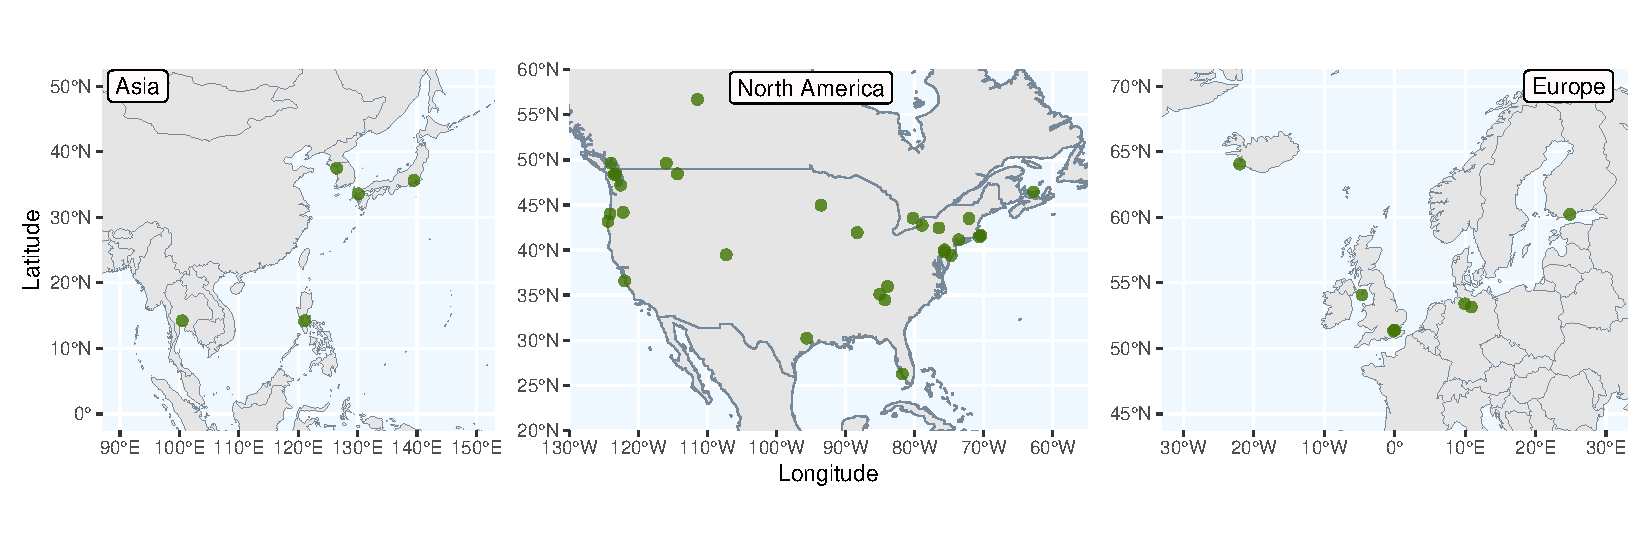
\includegraphics[width=1.01\linewidth]{fig1_gss_locs.pdf}
    \caption{The locations from which samples from good-performing turf were submitted to the Global Soil Survey from 2013 to 2016.}
    \label{fig:locs}
  \end{figure}

A total of 54 kits were received at the lab for analysis, producing test results from 162 locations with good performing turf. These samples came from 42 unique sites in ten countries on three continents (Figure~\ref{fig:locs}). There were more kits than sites because some participants purchased and submitted multiple kits. Summary statistics for the pH, soil organic matter, macronutrients, and secondary nutrients in these soils are shown in Table~\ref{tab:sumtable}.

\begin{table}
  \caption{Summary of Global Soil Survey data from September 2013 through August 2016. Five calcareous samples with pH > 7.7 and Mehlich 3 Ca > \SI{3000}{\mg\per\kg} were omitted from the summary analysis of Ca because the Mehlich 3 extractant dissolves some of the calcium carbonate in such samples.}
  \label{tab:sumtable}
  \centering
\begin{tabular}{lSSSSS}
  \toprule
{Soil parameter} & {n} & {Minimum} & {Median} & {Mean} & {Maximum} \\ 
  \midrule
pH & 162 & 4.6 & 6.5 &  & 8.2 \\ 
OM \si{\gram\per\kg} & 162 & 1.7 & 18 & 22 & 102 \\ 
  K \si{\mg\per\kg} & 162 & 10 & 60 & 73 & 296 \\ 
  P \si{\mg\per\kg} & 162 & 6 & 68 & 77 & 450 \\ 
  Ca \si{\mg\per\kg} & 157 & 125 & 586 & 834 & 4709 \\ 
  Mg \si{\mg\per\kg} & 162 & 23 & 76 & 90 & 516 \\ 
  S \si{\mg\per\kg} & 162 & 5 & 14 & 18 & 91 \\ 
   \bottomrule
\end{tabular}
\end{table}

Survey participants identified the sward composition to at least the genus level in 156 of the samples. Bentgrass (\emph{Agrostis} spp.), annual bluegrass (\emph{Poa annua}), and mixed stands of those grasses made up 110 of the samples. Other swards variously contained \emph{Cynodon} spp., \emph{Festuca} spp., \emph{Lolium perenne}, \emph{Poa pratensis}, \emph{Paspalum vaginatum}, and zoysia (\emph{Zoysia} spp.). Samples were also identified by use. Most samples came from golf course turf, with 100 coming from turf maintained as a putting green, 30 from fairways, 27 as tees, and 5 from turf maintained as sports fields or lawns.

We evaluated continuous probability distributions for their fit to these data and found the lognormal distribution had the best fit, based on the lowest values of the Kolmogorov–Smirnov statistic and on visual assessment of diagnostic plots.

The SLAN guidelines \parencite{clarifying-3} are for K, P, Ca, Mg, and S. The MLSN guidelines were developed for those same elements. Table~\ref{tab:sumtable} shows a summary of those same macronutrients and secondary nutrients found in the GSS data. In Table~\ref{tab:comparetable}, the minimum SLAN value is shown for each of those elements. The minimum SLAN value is the soil nutrient level at which no response to added fertilizer is expected based on the SLAN guidelines \parencite{clarifying-3}. The minimum values calculated for the MLSN data using log-logistic distributions, and for the GSS data using lognormal distributions, are also shown. The MLSN and GSS minimums come from evaluating the quantile function for the probability distribution at a value of 0.1.

 \begin{table}
    \caption{The GSS, MLSN, and SLAN guidelines. GSS and MLSN values are obtained by evaluating the quantile distribution of the distributions fit to the GSS and MLSN datasets at 0.1. The SLAN values come from \textcite{clarifying-3} and are the bottom of the high range, representing the soil nutrient content at which no grass response is expected from further additions of that nutrient.} 
\label{tab:comparetable}
  \centering
\begin{tabular}{lSSS}
  \toprule
{Element} & {GSS} & {MLSN} & {SLAN} \\ 
  \midrule
 K \si{\mg\per\kg} & 31 & 37 & 117 \\ 
  P \si{\mg\per\kg} & 23 & 21 & 55 \\ 
 Ca \si{\mg\per\kg} & 256 & 348 & 751 \\ 
   Mg \si{\mg\per\kg} & 36 & 47 & 121 \\ 
   S \si{\mg\per\kg} & 7 & 7 & 41 \\ 
   \bottomrule
\end{tabular}

\end{table}

The kernel density of survey results for pH, organic matter, and a suite of soil nutrients are shown in Figure~\ref{fig:density_gss}. We don't calculate minimum values for micronutrients or other soil parameters from these data. Rather, they are shown as descriptions of the nutrient levels and other soil test results from the GSS data.

   \begin{figure}
    \centering
    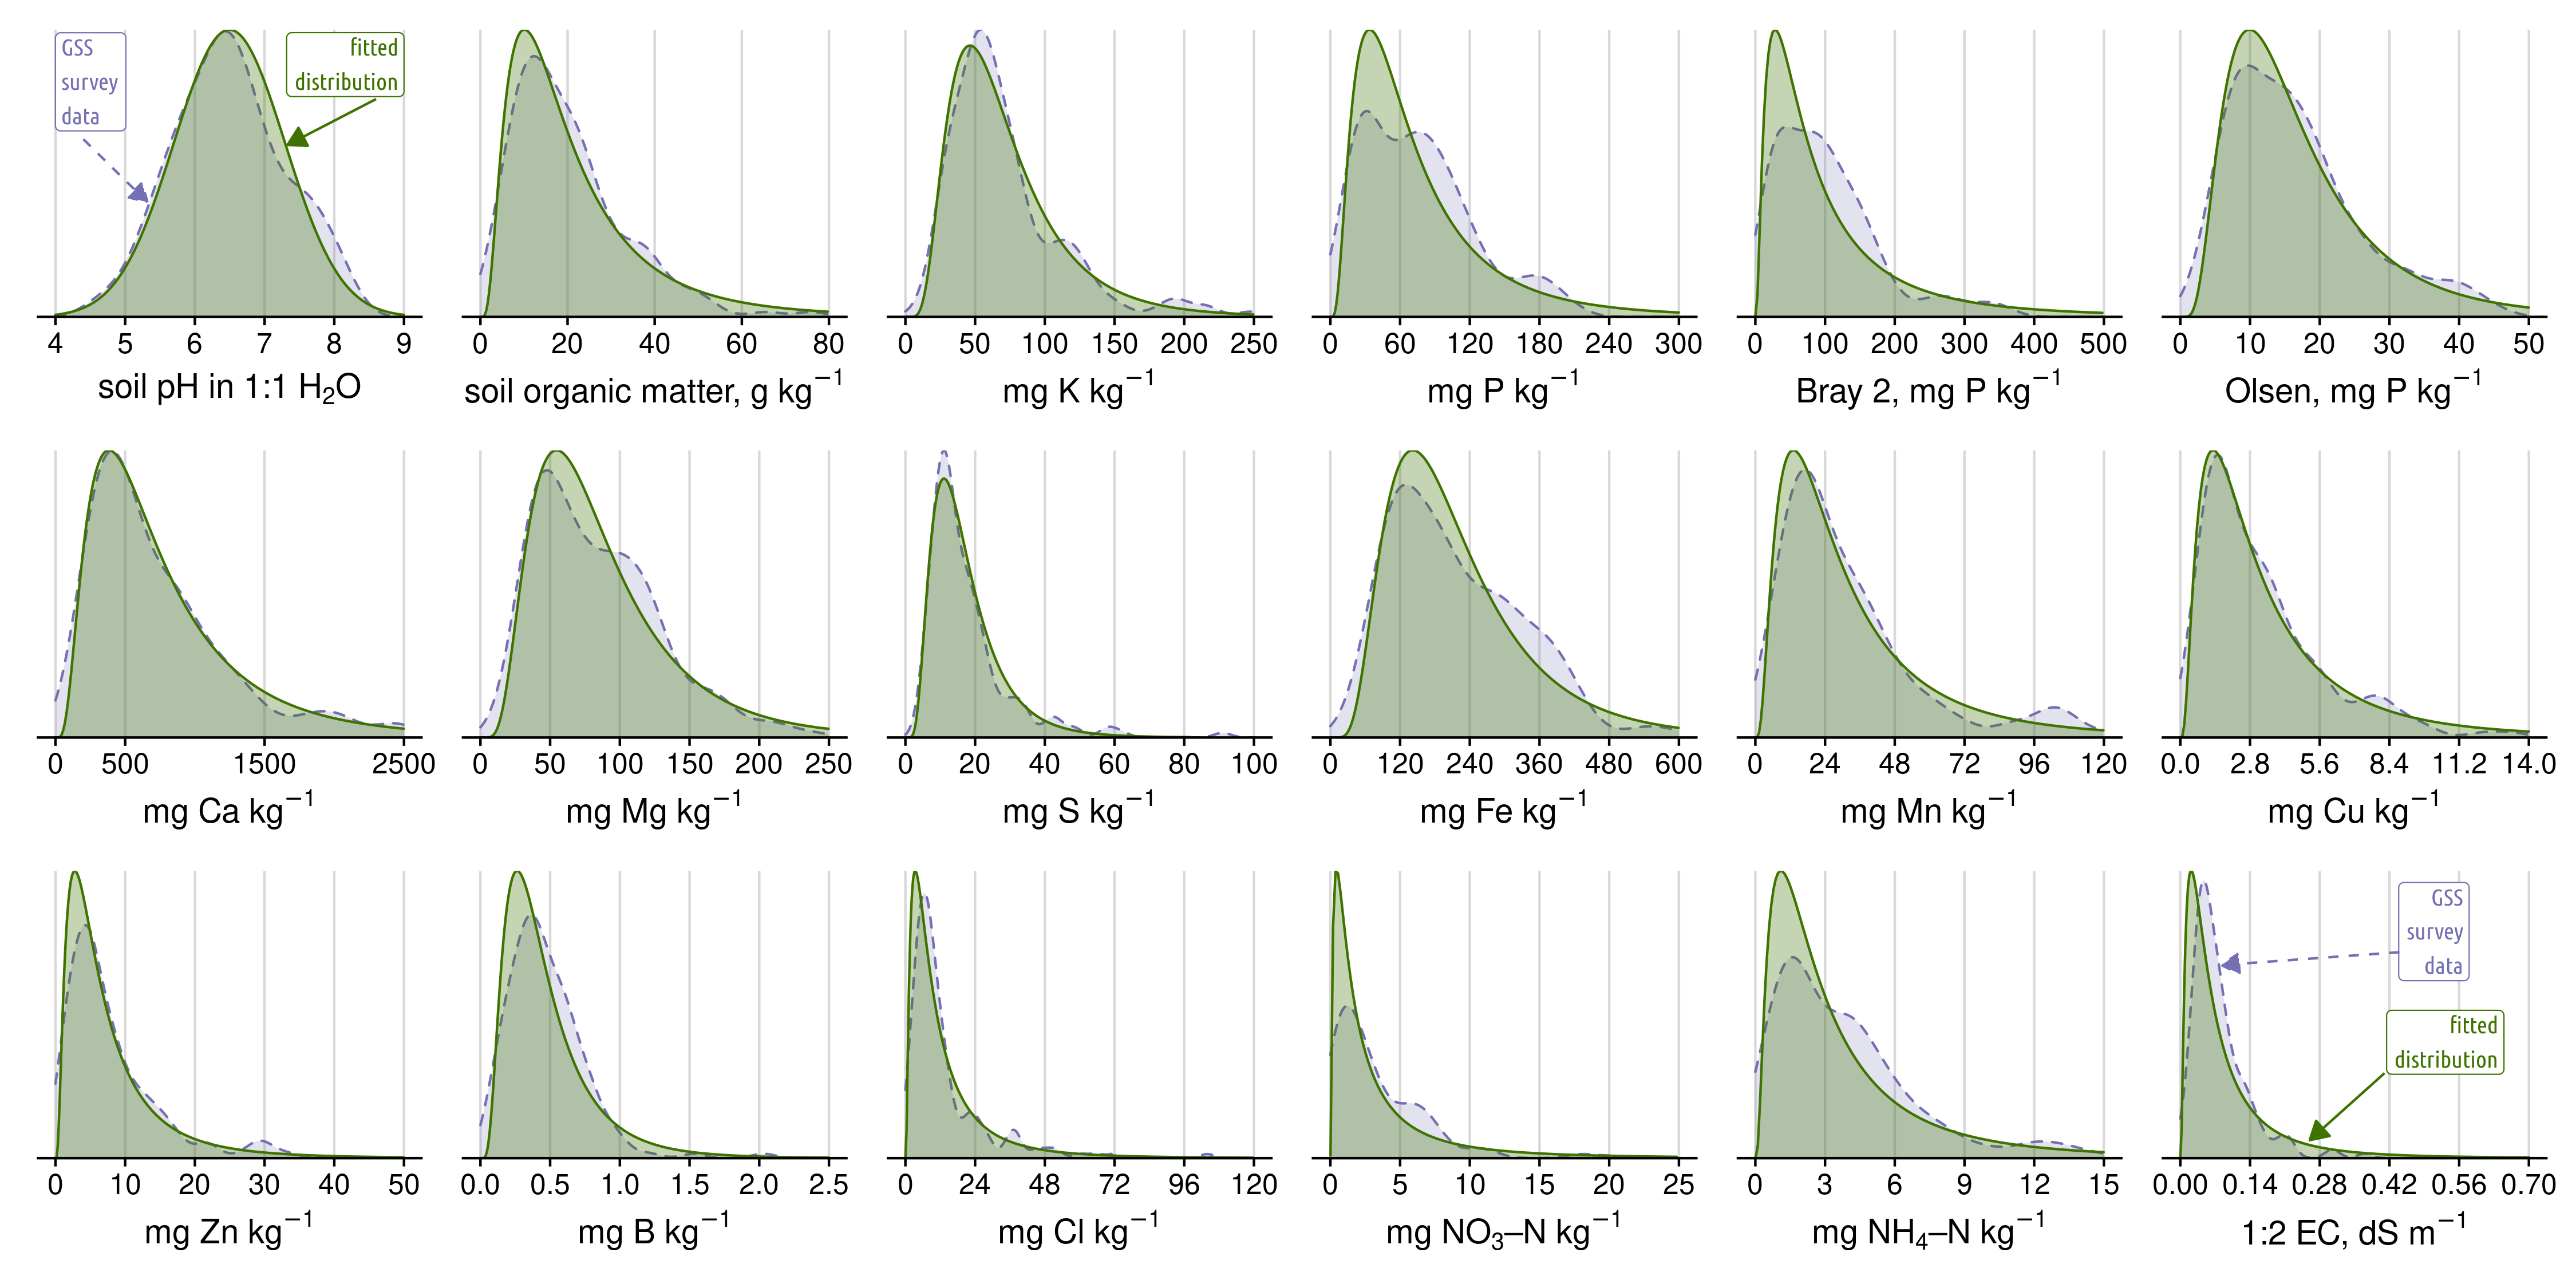
\includegraphics[width=1.01\linewidth]{fig2_survey_exact.png}
    \caption{Kernel density for Global Soil Survey data and for the distributions (normal for soil pH and lognormal for all other soil parameters) fit to the data.}
    \label{fig:density_gss}
  \end{figure}

  After fitting the lognormal distributions to the GSS data, we also plotted those distributions together with the log-logistic distributions that we fit \parencite{woods-peerj-2016} to the MLSN data (Figure~\ref{fig:density_both}). The distributions of the soil properties from good-performing turf in the GSS are similar to the properties from good-performing turf in the MLSN data.

     \begin{figure}
    \centering
    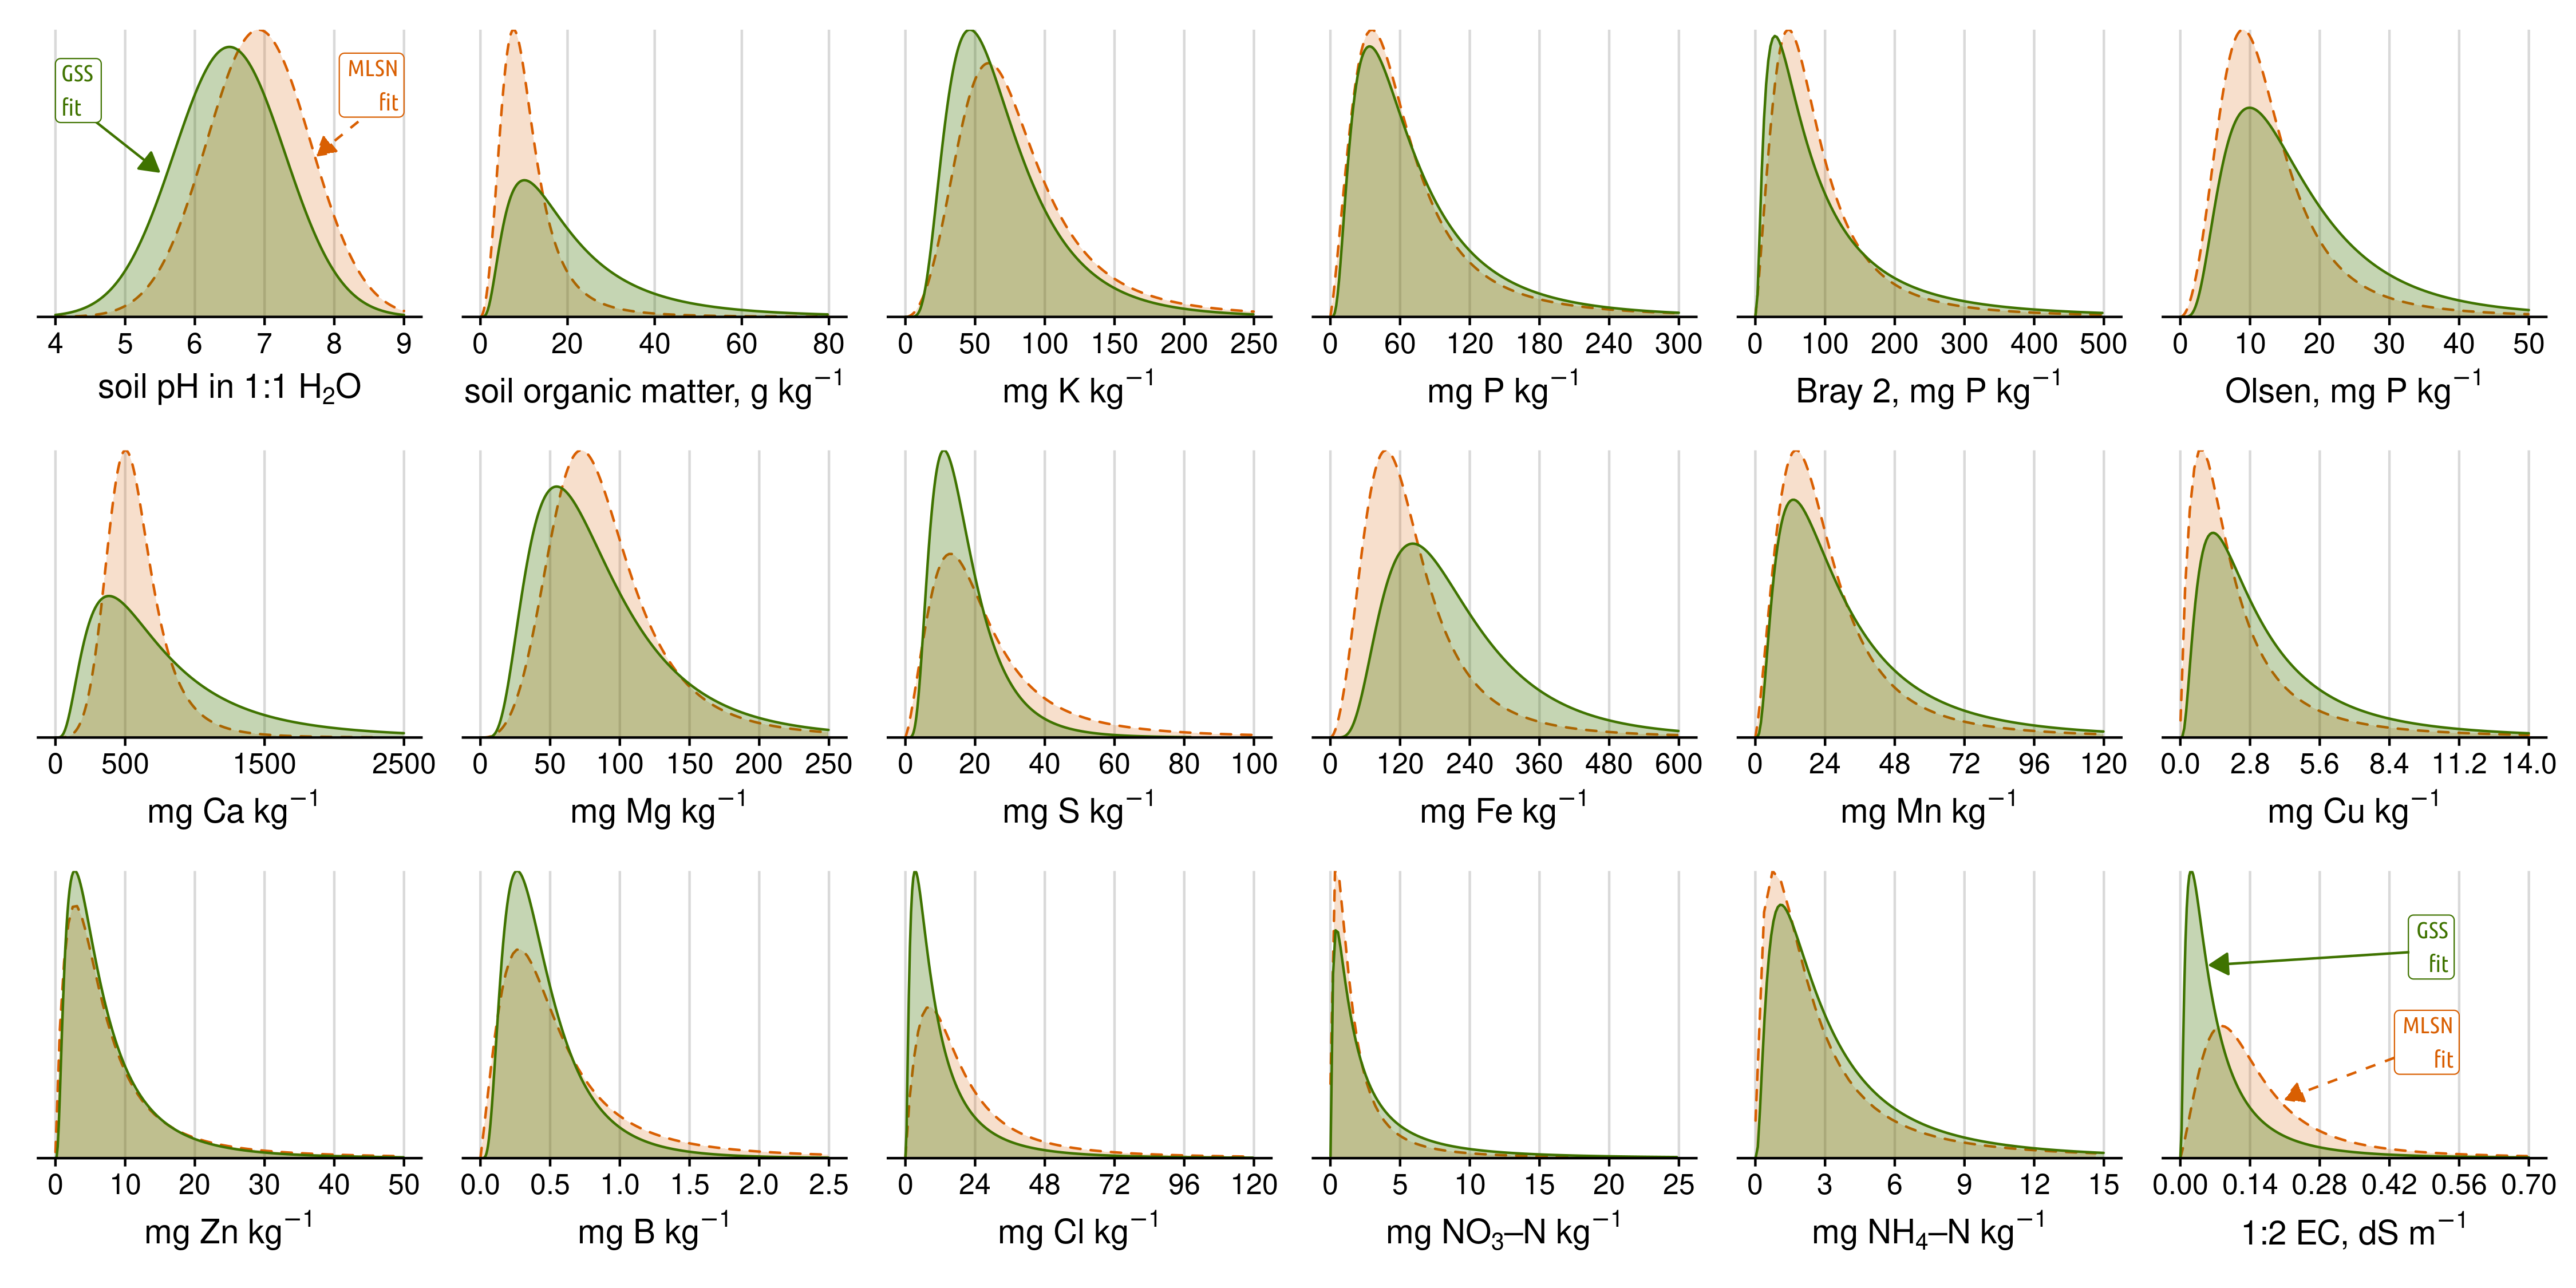
\includegraphics[width=1.01\linewidth]{fig3_compare_exact.png}
    \caption{Kernel density for lognormal distributions fit to the Global Soil Survey data and log-logistic distributions fit to the MLSN data.}
    \label{fig:density_both}
  \end{figure}

Lognormal distributions were fit to the GSS data with no filtering for pH and no filtering for estimated cation exchange capacity. This differs from the MLSN data, which had a log-logistic distribution fit to them after removing samples with pH less than 5.5 or pH greater than 8.5, and after selecting only soils with a cation exchange capacity by summation no greater than \SI{60}{\milli\mole\per\kg}. Even though the GSS data were unfiltered---except for the removal of five calcareous samples from the Ca data---the GSS data were generally lower than the filtered MLSN data. Kolmorgorov-Smirnov tests of the hypothesis that GSS data were larger than MLSN data---that the cumulative distribution function (CDF) of GSS data is above the CDF of MLSN data---had p-values less than 0.05 for K, Ca, Mg, and S. The exception was P, for which the GSS data were higher than the MLSN data. 

\section*{Discussion}

The GSS data suggest that good turf is being produced in soils with nutrient levels below those recommended by the conventional guidelines. \textcite{clarifying-3} described the SLAN low, medium and high ranges in these terms. If a soil tests in the low range, there is ``a high probability (80-100\%) that applying the nutrient will elicit a growth response.'' If a nutrient is in the medium range, there is ``approximately a 50\% chance of getting a plant growth response from application of the nutrient; if supplemental fertilizer is not applied, growth will probably be limited, especially as the season progresses.'' It is only when a nutrient is in the high range that ``little or no crop response is expected from applying the particular nutrient.''

The GSS data were collected from good performing turf. However, 34\% of the samples would be classified in the SLAN low range for K; 36\% low in Mg; 39\% low in Ca; and 52\% low in S. Using conventional soil test interpretation, we would expect more than a third of the GSS samples submitted to have an immediate growth response to added K, Mg, Ca, or S.

Phosphorus data in the GSS are distinct in being higher; 55\% of the GSS P samples would be classified as high by the SLAN guideline. In the high range---samples testing at Mehlich 3 P of \SI{55}{\mg\per\kg} or above---``little or no crop response is expected from applying the particular nutrient.'' Relatively high P seems common on turfgrass sites. \textcite{stansfield85} found ``excessive amounts'' of P in golf and bowling putting green samples tested from the UK and Ireland from 1978 to 1981. The MLSN data collected from 1991 to 2014 had a median Mehlich 3 P of \SI{53}{\mg\per\kg}. \textcite{landschoot2014} reported a median Mehlich 3 P of \SI{57}{\mg\per\kg} from 34,456 home-lawn samples in Pennsylvania from 2004 to 2009. The GSS P median was \SI{68}{\mg\per\kg}.

There appears to be an opportunity to reduce P fertilizer applications on some turfgrass sites, which can lead to reduced P leaching and runoff \parencite{bock2020, soldat2008}. The distribution of GSS P data matches closely the MLSN P data (Figure~\ref{fig:density_both}) that were used to derive the MLSN P guideline of \SI{21}{\mg\per\kg}. \textcite{kreuser2012}, \textcite{raley2013}, and \textcite{ogaard2020} have found values of soil P at a similar level are sufficient to produce good turf. 

The GSS data match well with the range and density of the MLSN data. The GSS data set is a small one, however, and there is some question about the consistency of the data if samples would be collected from more locations. There is also some expectation of selection bias in the GSS data. We consider it more likely that turf managers inclined to fertilize with a maintenance approach, supplying just what the grass requires, rather than those applying more fertilizer, would have participated in the GSS. We don't know how to quantify this but expect the GSS data to be biased somewhat lower than the results one would get by doing a random sample of good performing turf sites.

Comparing the GSS test results to the conventional guidelines provides an interesting result. Of the 162 GSS tests, each of which was collected from good-performing turf, 160 of them---99\% of the samples---had at least one macronutrient or secondary nutrient in the medium SLAN classification. According to SLAN, 99\% of the GSS samples would have a 50\% chance of responding to nutrient addition, right now. And 129 out of 162 GSS samples---a full 80\% of them---had at least one element in the low classification. Those soils would be expected, using SLAN recommendations, to respond immediately to fertilizer addition.

These GSS data can be used as a reference for normal nutrient levels, or normal soil test results, found in the rootzone of good-performing turfgrass. The GSS data cover a similar range as the MLSN data and suggest that the MLSN guidelines are reasonable for turfgrass across a wide geographic region.

\printbibliography

\end{document}
